\documentclass{article}

\usepackage{amsfonts}
\usepackage{amsmath}
\usepackage{amssymb}
\usepackage{amsthm}
\usepackage{caption}
\usepackage{color}
\usepackage{enumerate}
\usepackage{fancyhdr}
\usepackage[margin=1in]{geometry}
\usepackage{hyperref}
\usepackage{graphicx}
\usepackage{latexsym}
\usepackage{listings}
\usepackage{mathrsfs}
\usepackage[nottoc]{tocbibind}
\usepackage{setspace}
\usepackage{tikz}
\usepackage{tkz-graph}
\usepackage{url}

\providecommand{\all}{\ \forall \ }
\providecommand{\bs}{\backslash}
\providecommand{\e}{\varepsilon}
\providecommand{\E}{\ \exists \ }
\providecommand{\lm}[2]{\lim_{#1 \rightarrow #2}}
\providecommand{\m}[1]{\mathbb{#1}}
\providecommand{\mc}[1]{\mathcal{#1}}
\providecommand{\nv}{{}^{-1}}
\providecommand{\ov}[1]{\overline{#1}}
\providecommand{\p}{\newpage}
\providecommand{\q}{$\quad$ \newline}
\providecommand{\rt}{\rightarrow}
\providecommand{\Rt}{\Rightarrow}
\providecommand{\vc}[1]{\boldsymbol{#1}}
\providecommand{\wh}[1]{\widehat{#1}}

\hypersetup{
    colorlinks,
    citecolor=black,
    filecolor=black,
    linkcolor=black,
    urlcolor=blue
}

\pagenumbering{gobble}
\graphicspath{{../fig/}}

\begin{document}
\begin{flushleft}

\begin{figure}[htbp]
   \centering
   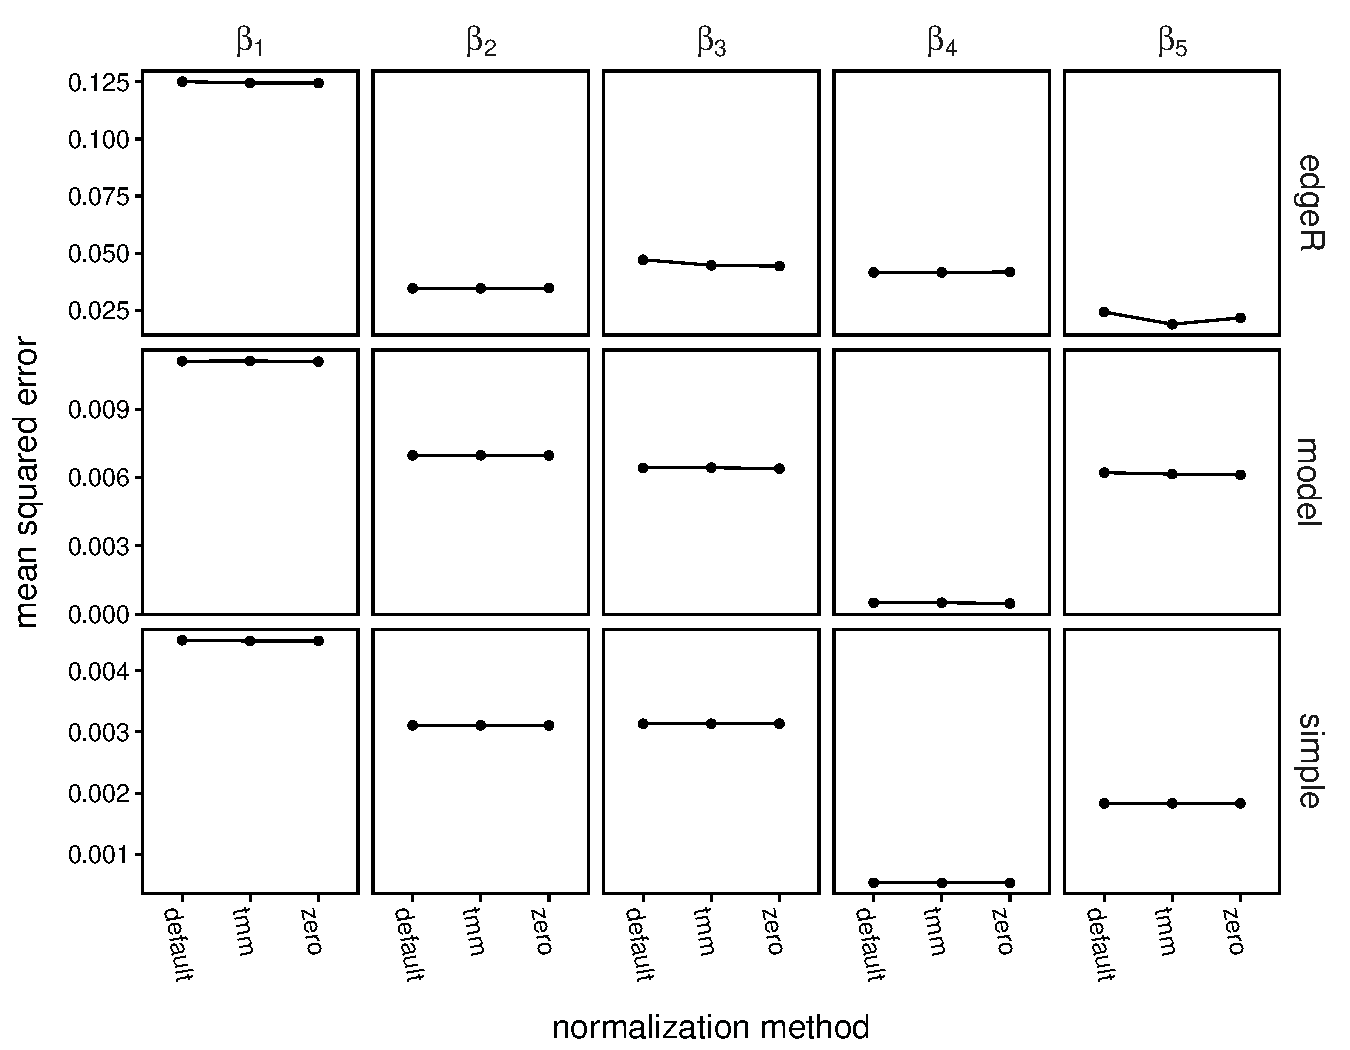
\includegraphics[scale=0.5]{mse}
   \caption{mse}
   \label{fig:mse}
\end{figure}

\begin{figure}[htbp]
   \centering
   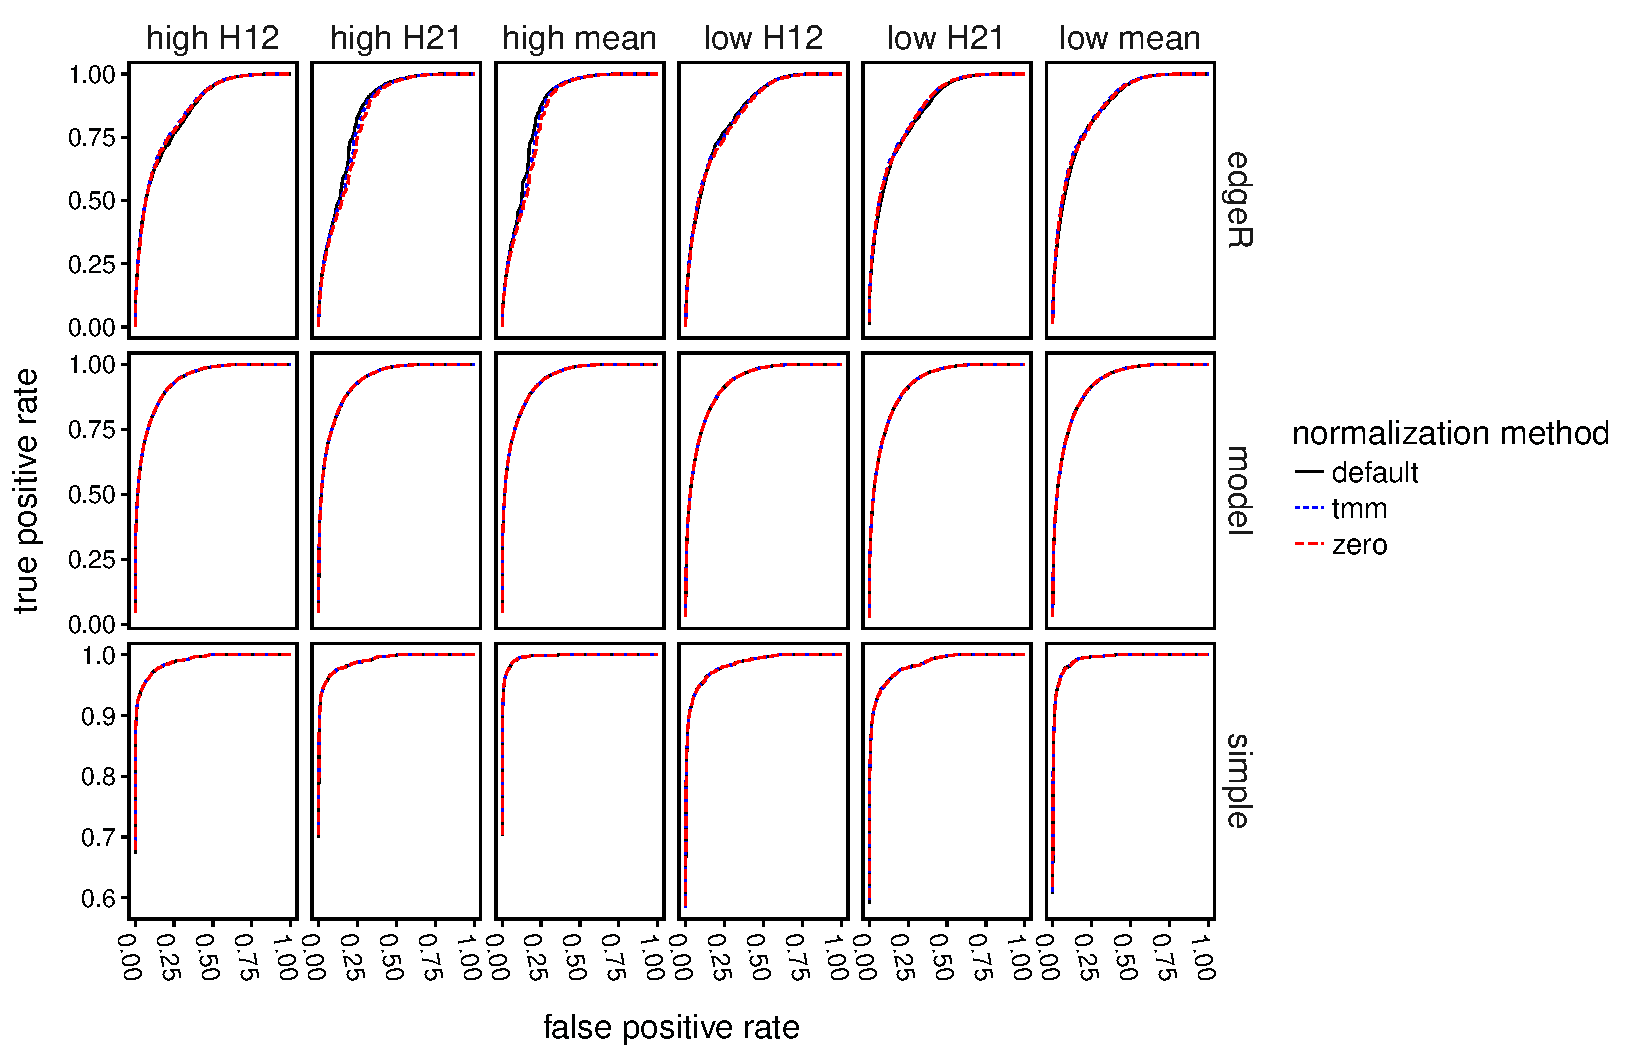
\includegraphics[scale=0.5]{roc}
   \caption{roc}
   \label{fig:roc}
\end{figure}

\begin{figure}[htbp]
   \centering
   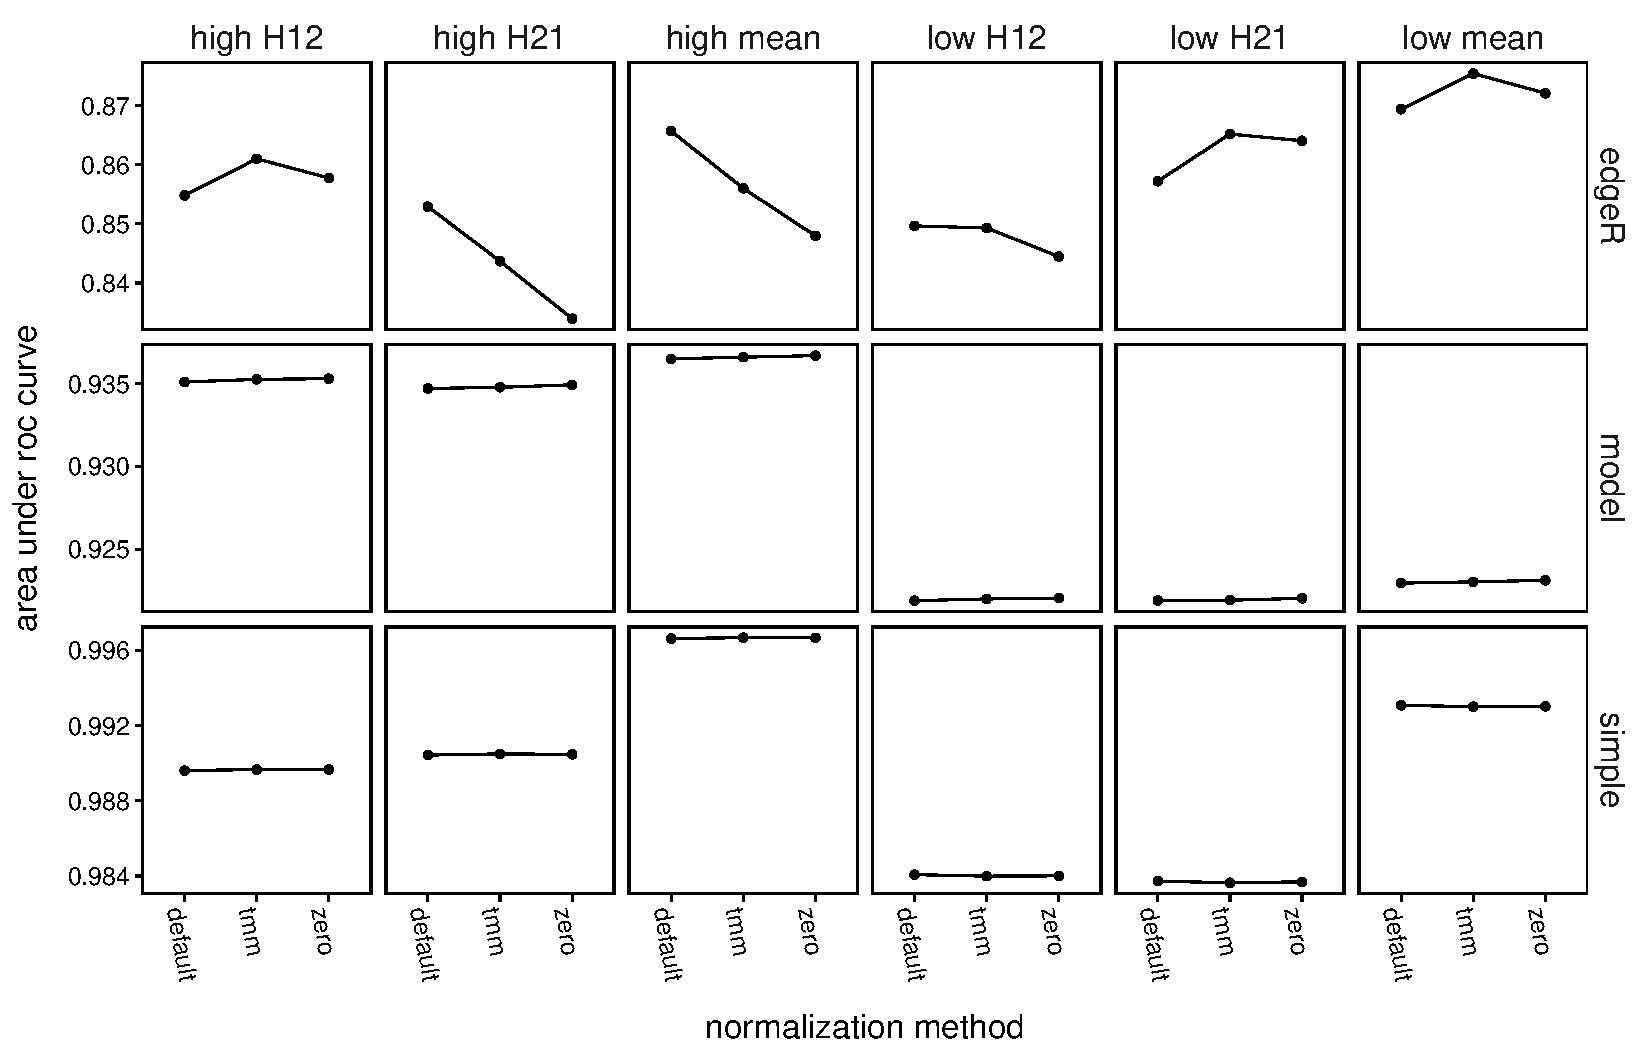
\includegraphics[scale=0.5]{auc}
   \caption{auc}
   \label{fig:auc}
\end{figure}

\begin{figure}[htbp]
   \centering
   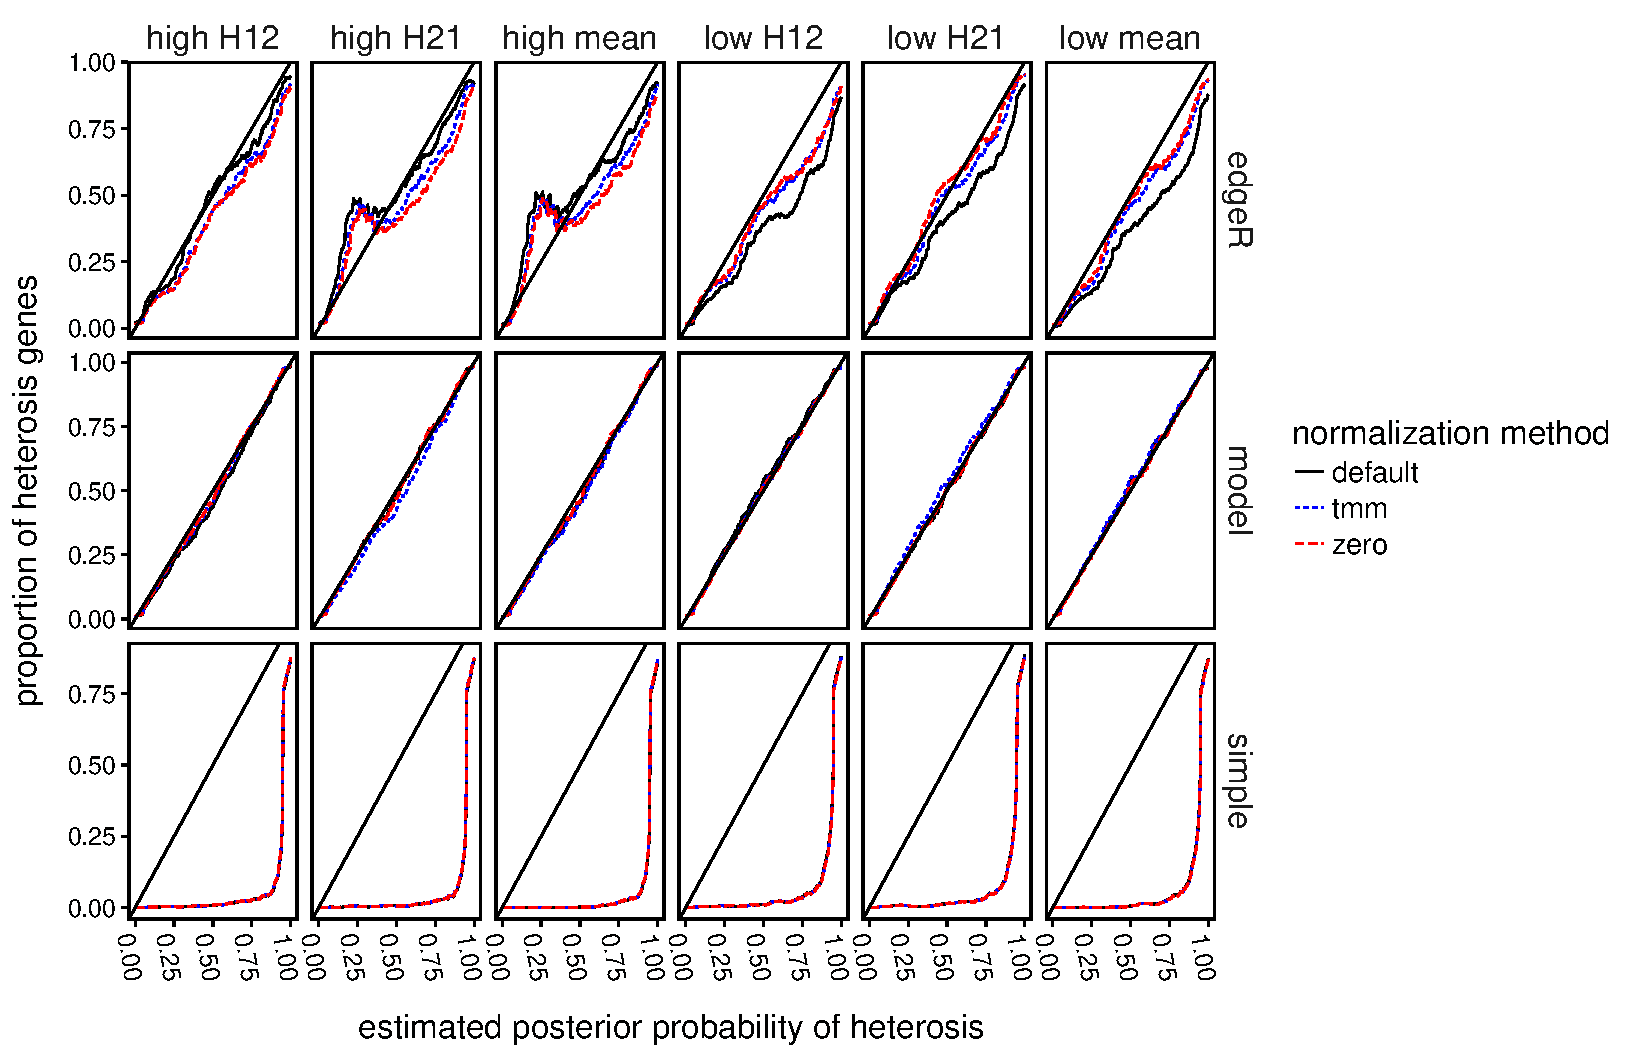
\includegraphics[scale=0.5]{calibration}
   \caption{calibration}
   \label{fig:calibration}
\end{figure}

\begin{figure}[htbp]
   \centering
   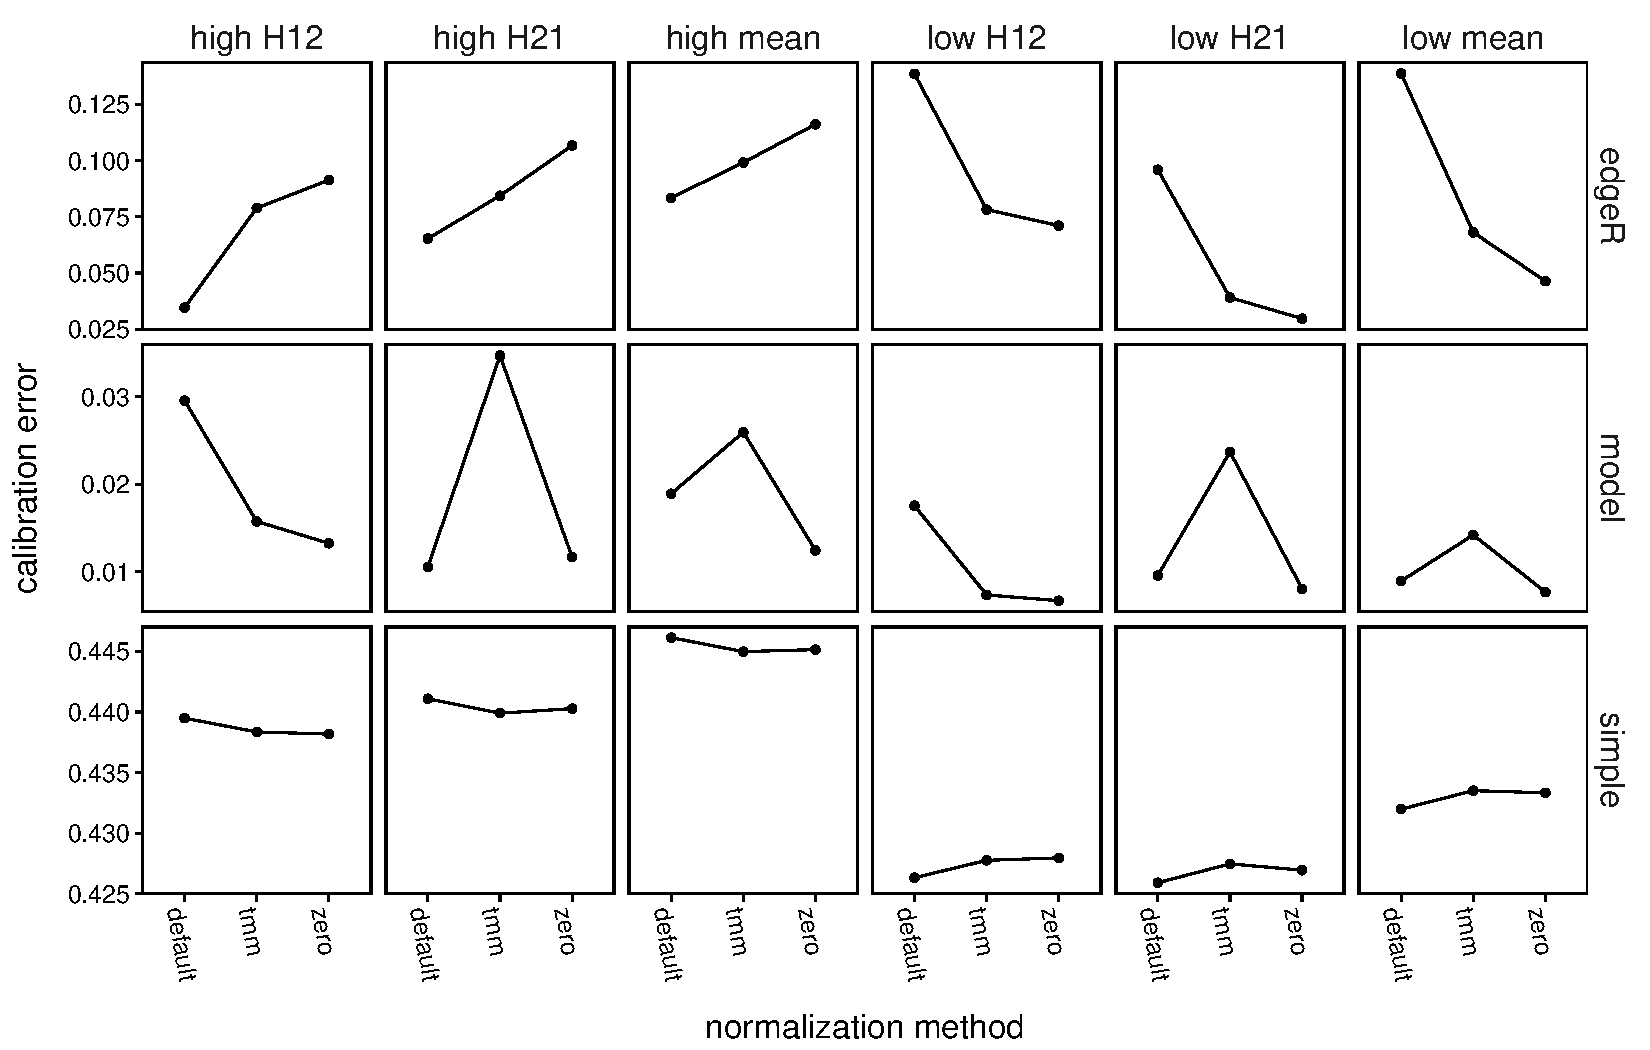
\includegraphics[scale=0.5]{calibration_error}
   \caption{calibration error}
   \label{fig:calibrationerror}
\end{figure}

\end{flushleft}
\end{document}